\documentclass[letterpaper,twocolumn,10pt]{article}
\usepackage{times}
%\usepackage[small,compact]{titlesec}
%\usepackage[small,it]{caption}
\usepackage{usenix}
\usepackage{endnotes}
\usepackage[tight]{subfigure}
\usepackage{natbib}
\setlength{\bibsep}{0.0pt}

\usepackage{url}
\usepackage{multirow}
\usepackage{array}
\usepackage{epsfig}
\usepackage{footnote}
\usepackage{amsmath}

\usepackage[compact]{titlesec}
\titlespacing{\section}{0pt}{*.4}{*.4}
\titlespacing{\subsection}{0pt}{*.4}{*.4}
\titlespacing{\subsubsection}{0pt}{*.4}{*.4}
\setlength{\parskip}{0pt}
\setlength{\parsep}{0pt}
\setlength{\headsep}{0pt}
\setlength{\topskip}{0pt}
\setlength{\topmargin}{0pt}
\setlength{\topsep}{0pt}
\setlength{\partopsep}{0pt}
%\widowpenalty=10000
%\clubpenalty=10000
%\setlength{\parskip}{0pt}
%\setlength{\dbltextfloatsep}{.2cm}
%\setlength{\dblfloatsep}{.2cm}
%\setlength{\textfloatsep}{.2cm}
%\setlength{\floatsep}{.2cm}
%\setlength{\topsep}{.2cm}
%\setlength{\intextsep}{.2cm}
%\setlength{\belowcaptionskip}{.2cm}
%\renewcommand{\topfraction}{0.85}
%\renewcommand{\textfraction}{0.1}
%\renewcommand{\floatpagefraction}{0.85}
%\hyphenpenalty=5000
%\tolerance=1000

\begin{document}

\title{\Large \bf On the Design and Implementation of Structured P2P VPNs}

\author{
David Isaac Wolinsky$^{\ast}$,
Linton Abraham$^{\bullet}$,
Kyungyong Lee$^{\ast}$,
Yonggang Liu$^{\ast}$,
\\
Jiangyan Xu$^{\ast}$,
P. Oscar Boykin$^{\ast}$,
Renato Figueiredo$^{\ast}$
\\
$^{\ast}$University of Florida, 
$^{\bullet}$Clemson University
\\
}

%\maketitle


\twocolumn[%
\centerline{\Large \bf On the Design and Implementation of Structured P2P VPNs}

\medskip

\centerline{\bf 
  David Isaac Wolinsky$^{\ast}$,
  Linton Abraham$^{\bullet}$,
  Kyungyong Lee$^{\ast}$,
  Yonggang Liu$^{\ast}$,
}
\centerline{\bf
  Jiangyan Xu$^{\ast}$,
  P. Oscar Boykin$^{\ast}$,
  Renato Figueiredo$^{\ast}$
}
\centerline{
  $^{\ast}$University of Florida, 
  $^{\bullet}$Clemson University
}
\bigskip
]

\subsection*{Abstract}
%\begin{sloppypar}
Centralized Virtual Private Networks (VPNs) when used in distributed systems
have performance constraints as all traffic must traverse through a central server.
In recent years, there has been a paradigm shift towards the use of P2P in
VPNs to alleviate pressure placed upon the central server by allowing participants
to communicate directly, relegating the server to handling session management and
acting as a relay when necessary.  Other approaches seek to remove all
centralization with a focus on unstructured P2P systems.
These approaches, currently lack the depth in security options provided
by other VPN solutions and have not been studied to understand the scalability of
using the system as a relay when NAT traversal fails.

To deal with these issues intuitively, we propose and implement a novel VPN
architecture using a structured P2P system for peer discovery, session
management, NAT traversal, and autonomic relay selection.  We relegate the use
of a central server as a partially automated  public key infrastructure (PKI)
via a user-friendly web interface.  Our model also provides the first design and
implementation of a P2P VPN with full tunneling support, whereby all non-P2P based
Internet traffic routes through a trusted third party.

In this paper, we describe the components of our model and evaluate our
reference implementation quantitatively to compare system and networking
overheads of the different VPN technologies focusing on latency, bandwidth,
and memory usage.  We also discuss some of our experiences with developing,
maintaining, and deploying such a system.
%\end{sloppypar}

\section{Introduction}
A Virtual Private Network (VPN) provides the illusion of a Local Area Network
(LAN) spanning over a public wide area network (WAN) infrastructure, guaranteeing
secure and authenticated communication amongst participants.  Common uses of
VPNs include secure access to enterprise network resources from remote/insecure
locations, connecting distributed resources from multiple sites, and
establishing virtual LANs for multiplayer video games over the Internet.  In
the context of this paper, we focus on VPNs that provide connectivity amongst
individual resources, all resources requiring symmetric connectivity will
be configured with VPN software.  Our work is significantly different
in scope from approaches that define VPNs ``as the `emulation of a private
Wide Area Network (WAN) facility using IP facilities' (including the public
Internet or private IP backbones).''~\cite{ip_vpns}.  In these VPNs,
large sets of machines are connected to a WAN-like VPN through one or
more virtual routers.

The architecture described in this paper addresses a usage scenario where
participants desire VPN connectivity without incurring the complexity or
management cost of traditional VPNs. For instance, in a small/medium business
(SMB) environment, it is often desirable to interconnect desktops and servers
across distributed sites and to provide authenticated access and encrypted
traffic to enterprise networked resources and Internet traffic from mobile
users at untrusted locations.  An example in academic environments is
collaboration amongst individuals belonging to a virtual organization
spanning multiple institutions, where coordinated configuration of network
infrastructure across different  sites is often impractical. Existing
approaches suffer from one or more limitations that hinder their
applicability in these scenarios: centralized approaches (e.g.
OpenVPN~\cite{openvpn}) incur the management cost of dedicated infrastructures,
while alternative P2P-based approaches (e.g. Hamachi~\cite{hamachi}) are
vulnerable to man-in-the-middle attacks if session management is handled by an
external provider and lack support for full VPN tunneling.

As we will present in this paper a centralized VPN can be a single point of
failure, can create a performance bottlenecks, and can compromise end-to-end
security.  While there have been several approaches to solve these problems,
\cite{openvpn, hamachi, wippien, p2pvpn, n2n, tinc} and more, as we will
show, there is not a single solution that provides the following desirable
traits:
user owned system for session management,
intuitive and user-friendly membership management of a VPN,
full tunneling of Internet traffic,
decentralized relay selection, and
the ability to handle large and distributed, active VPN pools.

Our system uses a freely available, automated public key infrastructure
(PKI).  The PKI is managed through a group-based web interface
that allows managers to review group join requests and remove malicious
users.  Furthermore, we bootstrap secure private P2P systems using existing
insecure public P2P system to avoid common trust concerns in P2P systems.
We explore the problem of providing full tunneling to P2P VPNs and provide
a working solution that supports multiple gateways in a single VPN.  We
provide mechanisms that allow two peers to establish two-hop links, relays, based upon
stability and proximity metrics when direct connectivity is unavailable.  The main
contribution of this paper is a novel structured P2P VPN overlay architecture,
while many of the individual components of our solution are not novel in
themselves, the integration of these components and their interaction results
in a unique system.

The rest of this paper is organized as follows.  Section~\ref{vpns} provides significant
details about VPNs by reviewing current VPN technologies.
Section~\ref{structured_p2p} reviews structured P2P systems.
Section~\ref{p2pvpn} describes the contributions of this paper, namely a feature-full
P2P VPN.  In Section~\ref{evaluation}, we verify our implementation through quantitative evaluation.
Our experience developing, using, and debugging the
system is presented in Section~\ref{experiences}.  In Section~\ref{related_work}, we
compare and contrast our work with related works.  Finally, we conclude in 
ection~\ref{conclusions}.

\section{Virtual Private Networks}
\label{vpns}
There exist many different flavors of virtual networking.  This paper focuses on
those that are used to create or extend a virtual layer 3 network, of which there
are many types, see Table~\ref{tab:vpn_types}.  A few popular
VPN showing the diverse categories are displayed in Table~\ref{tab:vpns}.
This section begins by going in depth on client configuration of VPNs, followed
by an overview of the different VPN server types.

\begin{table}[ht]
\setlength{\itemsep}{0pt}
\setlength{\parskip}{0pt}
\centering
\begin{tabular}[c]{|m{2cm}|m{5cm}|} \hline
Type & Description \\ \hline
Centralized & Clients communicate through one or more servers which are statically
configured \\ \hline
Centralized Servers / P2P Clients & Servers provide authentication, session management, and
optionally relay support while peers attempt to communicate directly with each
other, i.e., P2P links \\ \hline
Decentralized Servers and Clients & No distinction between client and servers,
each member in the system authenticates directly with each other, links between
members must be explicitly defined \\ \hline
Unstructured P2P & No distinction between clients and servers, members either know
the entire network or use broadcast to discover routes between each other \\ \hline
Structured P2P & No distinction between clients and servers, members are usually
within $O(\log N)$ hops of each other via a greedy routing algorithm, use 
distributed data store for discovery \\ \hline
\end{tabular}
\caption{VPN Classifications}
\label{tab:vpn_types}
\end{table}

\subsection{Client VPN Configuration}
\label{clientvpn}
In Figure~\ref{fig:vpn}, we abstract the common features of all VPNs clients.
The key components of a client machine are 1) client software that
communicates with the VPN overlay and 2) a virtual network (VN)
device.  During initialization VPN software starts by authenticating with an
overlay or VPN agent, then, optionally, it queries the agent for information
about the network such as the network address space, and finally the VN device
is started.

\begin{figure}[ht]
\centering
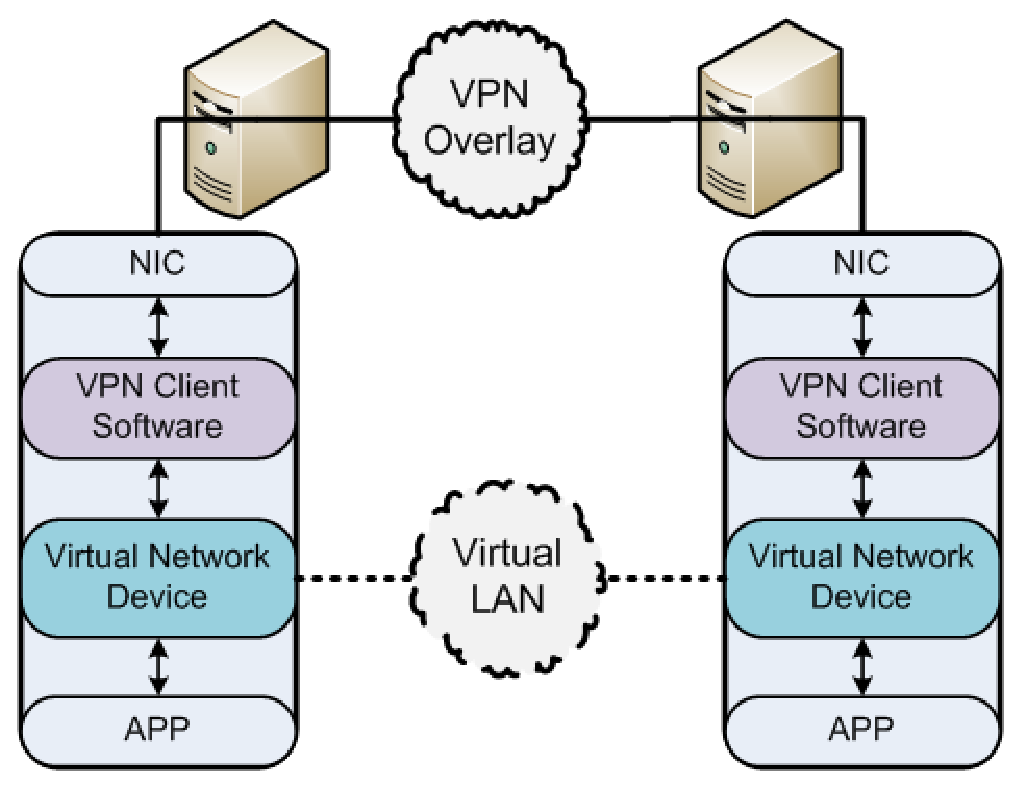
\epsfig{file=figs/vpn.png.eps, width=3in}
\caption{A typical VPN client.  The VPN uses a VN device to make interaction
over the VPN transparent.  Packets going to VPN destinations are
directed towards the VN device, which interfaces  the VPN client.
The VPN client in turn sends and
receives packets over the hosts physical network device.}
\label{fig:vpn}
\end{figure}

There are many authorization mechanisms for establishing communication with an VPN.
For quick setup, a system may require no authentication or use a shared secret
such as a key or password.  Uinsg accounts and passwords with or without a shared
secret provides Individualized authentication, allowing an administrator to block
all users if the shared secret is compromised or individual users if they act
maliciously.  For the strongest level of security, each client can be
configured to have a unique signed certificate that makes brute force attacks very
difficult.  The trade-offs come in terms of usability and management.  While the use of uniquely
signed certificates provides better security than shared secrets, it can be more
difficult to manage.  In a system comprising of non-experts, the
typical setup includes uses 
a shared secret and individual user accounts, where the shared secret is
included with the installation of the VPN application which is 
distributed from a secured site.

To communicate over the VPN transparently, a system must have a VN
device driver, which provide the mechanisms to inject incoming packets and retrieve outoing
packets and support the use common network APIs such as Berkeley Sockets allowing
existing application to work over the VPN without modification.
There are many
different types of VN devices, though due to our focus
on an open platform, we focus on TAP~\cite{tap}. TAP allows the creation of one
or more Virtual Ethernet and / or IP devices and is available for almost all
modern operating systems including Windows, Linux, Mac OS/X, BSD, and Solaris.
A TAP device exists as a character device providing read and write operations. 
Incoming packets from the VN are written to the TAP device and the networking
stack in the OS delivers the packet to the appropriate socket.  Outgoing
packets from local sockets are read from the TAP device.

The VN device can be configured manually through static addressing or
dynamically through dynamic host configuration process (DHCP)~\cite{dhcp0,
dhcp1}.  Setting of the address to the device causes the addition of a new
routing rule to the routing table that directs all packets sent to the
VPN address space to be sent to the VN device.  Packets are read from the
the TAP device, encrypted and sent to the overlay via the VPN client.
The overlay delivers the packet to another client or a server  with a 
VN stack enabled.  Received packets are decrypted, verified for authenticity,
and then written to the TAP device.  In most cases, the IP layer header remains
unchanged, while VPN configuration determines how the Ethernet header is handled.

The described configuration so far, creates what is known as a split tunnel,
or a VPN connection that only has passes \emph{VPN related traffic only and
not Internet traffic}.  Another form of tunneling exists called full tunneling.
Full tunneling allows a VPN client to securely forward \emph{all their Internet
traffic} through a VPN router.  This enables a user to ensure all their Internet
communication originates from a secure and trusted location and provides some
level of security when a user is an insecure and potentially hostile
environment, such as an open wireless network at coffee shop.  Both are visually
expressed in Figure~\ref{fig:tunnel}.

\begin{figure}[ht]
\centering
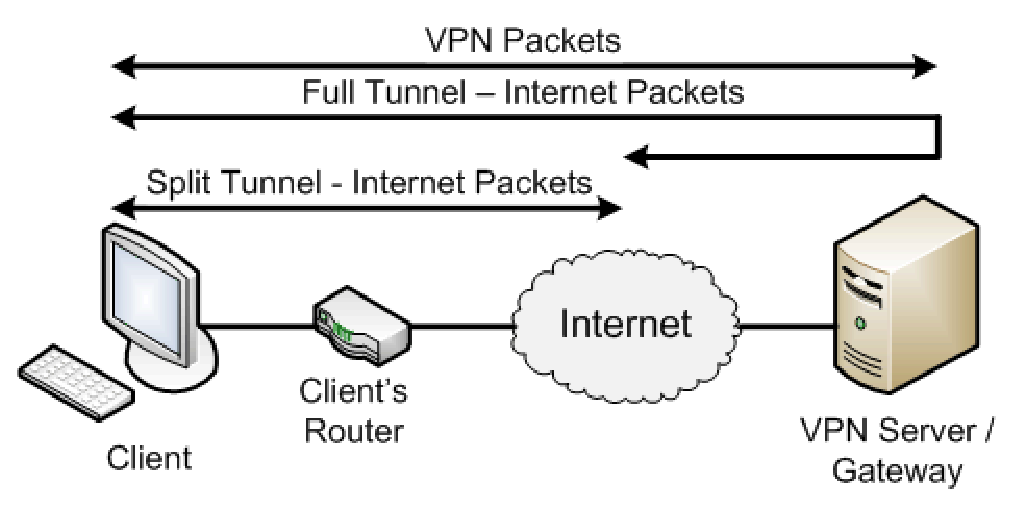
\epsfig{file=figs/tunnel.png.eps, width=3in}
\caption{A VPN setup expressing both full and split tunnel modes.  In both modes,
packets for the server are sent directly to the server.  In split
tunnel mode, Internet packets are routed directly to the Internet.  In full
tunnel mode, Internet packets are first routed to the server / gateway and then
to their Internet destination.}
\label{fig:tunnel}
\end{figure}

Most centralized VPNs implement full tunneling through a routing rule swap,
which makes the default gateway an endpoint in the VPN subnet and traffic
for the VPN server is routed explicitly to the LAN gateway.  In a 
typical home network, an Internet bound packet will be retrieved at the VN
device, encrypted, and sent to the VPN gateway via the LAN's gateway.  At the
VPN gateway, the packet is decrypted and delivered to the Internet.  All other
traffic is sent to the VN device, then sent securely to the VPN gateway.  A P2P
system provides two challenges:  1) P2P traffic must not be routed
to the VPN gateway and 2) there may be more than one VPN gateway.  We further
discuss this issue and provide solutions to this problem in Section~\ref{fulltunnel}.

%\small{
\begin{table*}[!h!t!]
\setlength{\itemsep}{0pt}
\setlength{\parskip}{0pt}
\centering
%\begin{tabular}[c]{|p{1.1cm}||p{3.475cm}|p{3.475cm}|p{3.475cm}|p{3.475cm}|} \hline
\begin{tabular}[c]{|m{2cm}||m{1.8cm}|m{2.4cm}|m{1.8cm}|m{2.9cm}|m{3.4cm}|} \hline
& VPN Type & Authentication Method & Peer Discovery & NAT Traversal & Availability \\ \hline \hline

OpenVPN~\cite{openvpn} & Centralized & Certificates or passwords with a central server &
Central server(s) & Relay through server(s) & Open Source\\ \hline

tinc~\cite{tinc} & Decentralized & PKI & Broadcast &
Relay through mesh & Open Source\\ \hline

CloudVPN~\cite{cloudvpn} & Decentralized & PKI & Broadcast &
Relay through mesh & Open Source\\ \hline

Hamachi~\cite{hamachi} & Centralized P2P & Password at central server & Central server &
NAT traversal and centralized relay & limited free-use, limited Non-Windows
clients, no private relays \\ \hline

GBridge~\cite{gbridge} & Centralized P2P & Password at central server & Central server &
NAT traversal, centralized relay & Windows only, freeware, no private relays \\ \hline

Wippien~\cite{wippien} & Centralized P2P & Password at central server & Central server & NAT traversal,
no relay support & Mixed Open / Closed source\\ \hline

N2N~\cite{n2n} & Unstructured P2P & Shared secret & Broadcast & NAT traversal,
decentralized relay & Open Source \\ \hline

P2PVPN~\cite{p2pvpn} & Unstructured P2P & Shared secret & Broadcast &
No NAT traversal, decentralized relay & Open Source \\ \hline

IPOP & Structured P2P & PKI or pre-exchanged keys &
DHT look up & NAT traversal and relay through physically close peers &
Open Source\\ \hline

\end{tabular}
\caption{VPN Comparison}
\label{tab:vpns}
\end{table*}
%}

\subsection{Centralized VPN Servers}
OpenVPN presents, as its name implies, an open and well documented method of implementing a
centralized VPN system.  While there may be minor differences amongst the
different centralized VPN implementations, it is our opinion that OpenVPN
provides a reasonable representation of features found in most centralized VPNs.
Centralized VPNs are responsible for authentication and routing between clients,
providing a NAT to the servers local resources and Internet (full tunnel), and
handling inter-server communication.

Central VPNs server operate at well-known endpoints known as
a universal resource identifier (URI) consisting of a hostname or IP address and
a port.  In a system containing multiple servers, a client attempting to log in
will randomly attempt to connect to one of the servers until
successful, implementing a simple load balance.  Once connected, clients obtain an
address in the VPN address space.  Depending on configuration this will allow a
client to communicate with other clients, resources on the same network as the
server, or Internet hosts via the VPN.  In such situations, it is important the
client and server both authenticate with each other in some form of challenge
response.

All inter-client packets flow through the central server.  In the default
configuration of OpenVPN, the clients encrypt the packet and sends to the server.
The server receives the packet, decrypts it, determines where to relay it, and then
encrypts and sends the packet to the its destination.  This model does not
prevent a server from eavesdropping on such
communication.  While a second layer of encryption is possible through a shared
secret, that requires
out-of-band communication and is less secure than relying on a PKI.

To support full tunneling or allow the client to access the server's resources,
the server too must enable client-like features by becoming a VPN endpoint with
a VN device.  Depending on the configuration, the server can than configure
traffic from the VPN to go through a NAT prior to routing it to the LAN and/or
Internet.  In Section~\ref{fulltunnel}, we present our configuration using
Linux and iptables, a layer 3 network stack manipulator.

OpenVPN allows a distribution of servers, so as to provide fault tolerance and
to a lesser degree load balancing.  Servers must be configured to know about
each other in advance and need routing rules established to forward packets.
Load balancing exists only in the process of the client randomly connecting to
different servers and potentially with a server refusing connection due to load.
There is no distributed load balancing.

Two examples of systems that assist in distributing load in VPN systems are
tinc~\cite{tinc} and CloudVPN~\cite{cloudvpn}.  Unlike the decentralized P2P
systems, these decentralized systems lack the ability to self-organize the VPN
overlay and require explicit description of links to create.  This
means that like OpenVPN, these systems can suffer VPN outages when nodes go offline.
The difference being that OpenVPN makes it explicit who is a server and who
is not, whereas in tinc and CloudVPN anyone can be a server or a client.  In the
typical tinc and CloudVPN setup, individual users share endpoints with each
other out-of-band, placing them in the VPN configuration file.  Due to
the lack of self-configuration, members in the system will not replace links
as members go offline.

\subsection{Centralized P2P VPN Systems}
Hamachi~\cite{hamachi} began the advent of centralized VPNs that went with the
ambiguous moniker ``P2P VPN''.  In reality, these systems would be best
classified as centralized VPNs servers with P2P clients.  Specifically, the
nature of P2P in these~\cite{wippien, gbridge} types of systems provides direct
connectivity between clients once authenticated by a central server.  While
direct connection is desirable, it does not always happen due to firewalls or
impenetrable NATs, when this happens, the central server either acts as a relay
or the two machines are unable to communicate.  One security consideration is
that each of these implementations use their own security protocols that
involve using a server to verify the authenticity and setup secure connections
between clients.  Most of
these projects are closed source not allowing users to host their own session
servers and relays, forcing the users to trust the third-party
server will not act as a man in the middle and eavesdrop.  None of these
provide support for full tunneling.

\subsection{P2P VPN Client / Server Roles}
\label{introp2p}
Unlike centralized systems, pure (or decentralized) P2P systems have no concept
of dedicated servers, though it is entirely possible to add reliability to the
system by starting dedicated instances of the P2P VPN.  In these systems, all
participants are members of a collective known as an overlay.  Current generation
P2P, decentralized VPNs use unstructured P2P networks, where there are no
guarantees about distance and routability between peers.  Two popular examples of
unstructured P2P VPNs are N2N~\cite{n2n} and P2PVPN\footnote{Due to the similarities
between the name P2PVPN and focus of this paper, P2P VPNs, all occurrences of
the string ``P2PVPN'' refer only to ~\cite{p2pvpn} and all occurrences of P2P VPN refer
explicitly to our research.}~\cite{p2pvpn}.  As a result
participants tend to be connected to a random distribution of peers in the
overlay.  Finding a peer requires either global knowledge of the pool or
broadcasting a look up message to the entire overlay.  While
unstructured P2P systems have some scalability concerns, P2P systems in general
allow for server-less systems.  The use of pure P2P ambiguates the role of client
and server, thus all clients are servers and all servers are clients.

Typically, decentralized, P2P VPNs begin by attempting to connect to well-known
endpoints running the P2P overlay software.  A list of such end points can be
easily maintained by occasionally querying the overlay for active participants
on public IP addresses and distributed with the application or some other
out-of-band mechanism.  In the case of P2PVPN, this involves communication with
one or more BitTorrent trackers to find other members of the P2PVPN group. 
N2N~\cite{n2n} requires knowledge of an existing peer in the system.  It uses
this endpoint to bootstrap more connections to other peers in the system,
allowing the application to be an active participant in the overlay and
 potentially be a bootstrap connection for other peers attempting to connect.

\section{Structured Peer-to-Peer Systems}
\label{structured_p2p}
Structured P2P systems provide distributed look up services with guaranteed
search time in $O(\log N)$ to $O(\log_2 N)$ time unlike unstructured systems
that must either know all the state in the system or make random walks
\cite{unstructured_v_structured}.  Some examples of structured systems can be found
in~\cite{pastry, chord, symphony, kademlia, can}.  In general, structured
systems, are able to make these guarantees by self-organization, whereby a node
entering the system follows some form of these abstracted steps:
generates or obtains a unique identification number (node ID) on the
order of 128-bits to 160-bits,
connects to random addresses on a pre-shared well-known endpoints list,
becomes connected to at least one peer in the list (leaf connection),
finds the peers closest in the address space to its node ID, connects
to the one immediately smaller and / or larger than itself (neighbors),
and finally connects to other nodes in the ring that are not local in the address
space (shortcuts).

The node ID must be unique to each peer, otherwise there will be an address
collision and the two peers will attempt to connect with the same set of peers.
The peers will only connect to one of them creating instability.  Furthermore,
having the node IDs well distributed will assist in providing better scalability
as many algorithms for selection of shortcuts depend on having node IDs uniformly
distributed across the entire node ID space.  A simple mechanism to ensure this
is to have each node use a good, cryptographically strong random number
generator.    Applying the birthday problem in this context would require
between $2^{64}$ to $2^{80}$ peers in a system for there to be a 50\% chance of
address collision.  Another mechanism for distributing node IDs involves the use
of a trusted third party to generate node IDs and cryptographically sign
them~\cite{secure_routing}.

Similar to the case of unstructured P2P systems, the incoming node must know
of at least one participant in the system in order to connect to the system.  To
summarize what was stated in Section~\ref{introp2p}, a list of nodes that are
running on public addresses should be maintained and distributed with the
application or be available through some out-of-band mechanism.  Other proposals
suggest using multicast to find pools~\cite{pastry}.  This can work well in
certain environments but multicast range can be quite limited.

Depending on the protocol, a node must be connected to either the closest
neighbor smaller, larger, or both.  Optimizations for fault tolerance suggest
that it should be between 2 to $\log(N)$ on both sides.  If a peer does not
know of the address of its immediate predecessor or successor and a message
is routed through it destined for them, depending on the message type, it may
either be locally consumed or thrown away, never arriving at its appropriate
destination.  Thus having multiple
peers on both sides assist stability when the system is experiencing churn,
especially when peers leave without warning.

Shortcuts make quickly traversing a P2P structure possible.  There are many
implementations and proposals for determining shortcuts, each has differing
costs associated.  A few of these include:  maintaining large tables without
using connections and only verifying usability when routing
messages~\cite{pastry, kademlia}, maintaining a connection with a peer every
set distance from you in the P2P address space~\cite{chord}, or using a handful
of well calculated locations in the node ID space~\cite{symphony}.

\section{Components of a P2P VPN}
\label{p2pvpn}
Before presenting our contributions made in this paper, we first review our
current work as it provides the basis for our P2P VPN.  At the heart of our
system lies a P2P system similar to Symphony~\cite{symphony}, named
Brunet~\cite{brunet}.  The specific components of the system that make it
interesting for use in a P2P VPN system include: NAT traversal~\cite{brunet},
system stability when two nodes next to each other in address space cannot
directly connect~\cite{hpdc08_0}, proximity based selection of shortcuts~\cite{hpdc08_0},
a distributed data store based upon a distributed hash table~\cite{pcgrid07},
and self-optimizing shortcuts to support single-hop connectivity between peers
in the overlay~\cite{wow}.

Furthermore, we have implemented a VN with the
following features: self-configuring, low overhead use~\cite{sc09, ipop},
discovery of members through the use of a virtual DHCP server using DHT~\cite{sc09, pcgrid07},
scalability in the count of hundreds of peers in a single VN~\cite{sc09},
portability to any system that supports Tap and Mono\footnote{
Mono is an open source implementation of .Net also known as the Common Language
Run-time (CLR), which provides managed run-time environment similar to Java.}~\cite{mono},
ability to behave as a VN interface or router~\cite{sc09},
secure end-to-end (EtE) and point-to-point (PtP) links,
and use in grid computing for over 3 years~\cite{archer,vtdc,pcgrid08,gridappliance}.

While this framework provides the basis for our design and implementation, we will show
in this paper that these components are abstract enough to be applied to other systems.

\subsection{Security through Groups}
Our VPN supports the PKI model, where a centralized CA signs all client
certificates and clients can verify each other without CA interaction by using the CA's public
certificate.  Setting up, deploying, and then maintaining security can easily
become a non-negligible task.  Most PKI-enabled VPN systems 
require the use of command-line utilities, setting up your own methods of
securely deploying certificates, and policing users.  Our experience with users
indicate that usability is very important, which is why we sought a model with
easy to user interfaces.  In this section, we
present our solution, a partially automated PKI reliant on a redistributable group based web
interface.  Although this does not preclude other methods of CA interaction,
we believe it provides a model that will be satisfactory for many use cases.

In order to obtain certificates, a user creates an account an joins a group,
providing relevant information as to the reason for joining the group.  Where
upon an administrator can verify this information and approve or deny the user
access into the group.  If a user is granted access, they are then able to
download a configuration blob that uniquely identifies them and allows them to
automatically get certificates in the future.  The user configures the VPN
client with the binary blob.  Upon starting, the VPN client queries the group
server using the information in the blob to authenticate the server and itself to
the server.  After which, the user provides the group server a certificate
request containing the VPN clients node ID, which the server signs and returns.
At which point, the VPN client and connect to the VPN pool and communicate
securely with others in the group.  It is imperative that any operations that
involve the exchanging of secret information, like the blob, be performed
over a secure medium, such as HTTPS, which can be done with no user
intervention, otherwise, the blob can become a security issue.

Unlike decentralized systems that use shared secrets, in which the creator of
the VPN becomes powerless to control malicious users, a PKI enables the creator
to maintain order in the VPN and remove malicious users.  The methods that we
have incorporated include:  use of a certificate revocation list (CRL) hosted
on the group server, DHT events requesting notification of peer removal from
the group, and broadcasting to the entire P2P system the revocation of the peer.

A CRL offers an out of band mechanism for distributing user revocations, unlike
information exchanged in a P2P overlay, primarily because malicious users can
use common P2P attacks to prevent notification of certificate revocations
transmitted via the overlay, but it is significantly more difficult to prevent
the retrieval of a CRL.  Furthermore, if a client is unable to retrieve the
latest CRL, it will be clear that there is a connectivity issue with the CRL
server and it can act appropriately, depending on the security requirements.
The downside is that the CRL is centralized and it can be prohibitively
expensive for peers to verify certificates on regular intervals with short
periods.

The DHT method acts as a event notification.  Users place their a their
node ID into the DHT at a key specific to a peer they are communicating with.
Upon revocation, the group server reads the values at this key and notifies
all client of the revocation.  The problem with a
DHT is that it can be easily compromised if they have not been implemented
with significant measures to protect against maliciousness.

The most rudimentary mechanism is broadcasting the certificate
revocation over the entire P2P overlay.  In small networks, the cost of such a
broadcast may be negligible, but as a network grows, such a broadcast may
become prohibitively expensive.  A broadcast can be harder to block
as a malicious node would need to have significant collusion
in order to completely interrupt the broadcast, though this is feasible in our
model if groups use automated certificate signing.  Furthermore, the broadcast
acts similarly to the DHT event notification, as such, peers find out on a push
like mechanism.  

\subsection{Full-Tunneling over P2P}
\label{fulltunnel}
As discussed in Section~\ref{clientvpn}, VPN tunneling is divided into two
categories:  split tunneling and full tunneling.  In split tunnel mode, the
the VPN client receives and sends messages related only to the VPN, i.e., both
end points are in the VPN; whereas in full tunnel mode, all traffic both VPN
and Internet traffic with the exception of VPN ``control'' messages route over
the VPN, as shown in Figure~\ref{fig:tunnel}.
In a centralized VPN these ``control'' messages would be the
communications directly with the VPN server and full tunnel gateway, which most
likely is the same machine destination IP address from the perspective of the
client.  In a P2P VPN, ``control'' messages would be communications directly
between P2P peers.  Using full-tunneling ensures that a malicious user cannot
easily eavesdrop into what would otherwise be public communication by
forwarding all non-VPN related traffic securely to a third party who resides
in a more trusted environment.  There are two key components to this scheme,
a gateway / server or traffic relayer and a client or a traffic forwarder.
In the following sections, we present a methods for implementing
gateways and clients.

\subsubsection{The Gateway}
Configuring a machine as a gateway can be done with NAT software, in Linux
this is possible through iptables.  One of the components in iptables that
provides NATs is called masquerade, which automatically handles forwarding
packets received on one interface and to the next hop as well as receiving
packets from the Internet and forwarding them back to the appropriate client,
transparently taking care of NAT.  Use of existing NAT software is recommended,
as many applications, including FTP and SIP, embed IP information into the data
of packet, making IP header manipulation insufficient for NAT support.

With a gateway intact, the VPN software can now announce that it provides
full tunneling.  For that purpose, we added an enable flag into the VPN
configuration to specify that a machine is a full tunnel gateway.  When the
VPN software starts, it will automatically append itself to the list of known
gateways for the VPN group in the DHT.

The only remaining difference in VPN gateway is the state machine used in
processing packets coming from the VPN.  Previously, packets were rejected
if the destination was not in the VPN subnet, now they are only rejected if
gateway mode is disabled.  If it is enabled, all packets are written to the
TAP device with the destination Ethernet address being that of the TAP device.
The remaining configuration is identical to other members of the system as
packets from the Internet to the client will automatically have the clients
IP as the destination as a product of the NAT.

\subsubsection{The Client}
VPN Clients wishing to use full tunnel must redirect their default traffic to
their VN device.  In our VPN model, we use a ``virtual'' virtual address for
the purpose of providing distributed VN services DHCP and DNS.  This same
address can be used as the VPN gateway, which works fine because as shown in
Figure~\ref{fig:tunnel_packet}, only the Ethernet header contains information
about the gateway.  Packets retrieved in the VPN software can then
forward the Internet packet to any machine in the VPN providing gateway services
without changing IP or higher OSI layer changes.

The VPNs state machine has to be slightly modified to handle outgoing packets
not destined for a remote VPN end point.  Incoming packets destined for a subnet
outside of the VPN address space will be rejected, unless full tunnel client mode
is enabled.   If it is enabled, the VPN software finds a remote peer to act as a
full tunnel gateway and then send the packet to the remote peer.

\begin{figure}[ht]
\centering
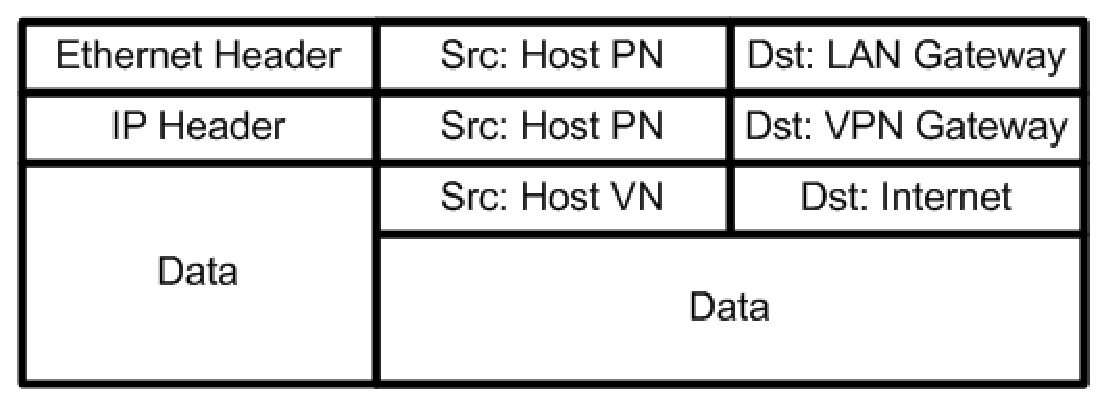
\epsfig{file=figs/tunnel_packet.png.eps, width=3in}
\caption{The contents of a full tunnel Ethernet packet.  PN and VN are defined
as physical and virtual network, respectively.  Interesting components of this
packet are 1) the destination Ethernet address is the LAN gateway, 2) the
destination IP address is the VPN gateway, and 3) the IP payload contains
another IP packet whose source IP is the VN device and destination is the
Internet.}
\label{fig:tunnel_packet}
\end{figure}

The pathway for packets coming from the overlay needs some tweaking as well.
The source IP address will not match the VPN gateways IP but rather the Internet
address.  Thus the VPN client must confirm that the source is a VPN gateway, if
not the packet is thrown away.  Upon writing a packet to the VN device, the user
application will have appeared to receive a packet from the Internet.

This leads to two issues, how to select the machine to use as a gateway and how
to configure a network stack to properly route packets and not direct all packets
to the VPN gateway.  Our model uses a simple mechanism for determining
which gateway to choose:  query the DHT for a list of potential gateways, select
a random one from the list, and verify liveness via periodic (15 second interval)
ping messages.  For handling faults, we take a pessimistic approach, that is,
if a server is lost, we take note of it and only query the DHT again upon the
next outgoing Internet packet.

In this paper, we focus on the second issue, handling P2P routed packets.
In the centralized VPN case, a client communicates directly
with a single point in the VPN, which is known ahead of time and can be implemented
by a simple routing rule swap prior to starting the VPN.
The same cannot be done for a P2P system.  Due to the nature of P2P systems,
ensuring that all P2P overlay messages are routed directly
becomes a non-trivial issue as there will be many such routes most of which will
not be known ahead of time.  If we applied the same model used by centralized VPNs,
the client would end up routing both Internet and P2P traffic through the gateway
machine creating a central point for failure and removing the advantage of P2P,
scalability.  To solve this we present two approaches though in our efforts, we
were only successful with one model for easily setting up a client.  We
present all our work, including our failed attempt, such that it may be the
ground work for further research.

\subsubsection{The Client -- Approach 1 -- Adding Routes}
The first approach is similar to the centralized version,
for each P2P link, we add an explicit rule in the
routing table so that packets destined for those endpoints are routed directly to them via
the LAN's default gateway.  In order to ensure this, we added a feature to the
socket handling code that would prior to the first outgoing packet
indirectly add a routing rule to direct packets for the remote nodes
public address to the LAN gateway.  The rule would remain in effect until the
VPN closed down or the link was closed.
This model requires unique code for each OS platform, though supporting
Linux and Windows was quite trivial.
Because outgoing packets bear the source address of the physical network,
incoming packets will be delivered normally.

This method has two major flaws.  Common to all VPNs that employ
the standard route switch technique, all communication, not just VPN, is routed
directly to the server insecurely.  So while the VPN traffic is most likely
encrypted, if the server also hosts a website, that traffic will be in its natural
state, potentially unencrypted, and visible to any eavesdroppers.  An issue,
unique to our P2P solution, allows a malicious user to send spoofed packets
to have the VPN which will add extra routes to the routing table, resulting in a similar
situation as the first, unencrypted communication visible to eavesdroppers.

\subsubsection{The Client -- Approach 2 -- Ethernet Packets}
This solution attempts to solve the problem introduced by the first solution,
removing any potential for eavesdropping.
This approach recognizes that when using UDP or TCP an application can determine
the source ports from which all application traffic would originate.
This approach requires the routing rule directing all traffic to
the VPN gateway, though there are no additional routing rules.  This results in
all packets being directly sent VN device, leaving the VPN client software to handle
Ethernet layer routing of the packets.

When packets come into the VPN application, the client checks the source port,
if it matches one of the applications source ports, the VPN client must
change the source IP address to match the hosts LAN IP address and then embed
the packet into an Ethernet frame prior to sending it to the local gateway.
Cross platform components that allow writing Ethernet frames to physical host
network devices include using a bridged tap device whose sole purpose is to
send and receive Internet packets to and from the gateway and using
PCap, a packet capture and injection library, to send packets.

The problem with this approach is that when an incoming packet arrives at the
clients networking stack, the client does not recognize the packet because the
destination IP address does not match the original outgoing address as the
packet is destined for the physical Ethernet's IP address and not the VN Ethernet's.
This triggers the OS to either ignore the packet, UDP, or send a TCP reset message.
Thus the solution needs some form of NAT, that would handling receiving incoming
packets and rewriting them prior to the network stack thus avoiding a TCP
reset message, a task we have not yet investigated.

\subsection{Autonomic Relays}
A handful of P2P VPNs~\cite{hamachi, gbridge} support relaying when direct
communication is not possible though a majority of them do not~\cite{wippien}.
Centralized and decentralized VPNs do not suffer from this problem
as all traffic passes through the central server or managed links.  To address
the management and overhead concerns presented these systems, we propose
the use of distributed, autonomic relaying system based upon previous
work known as ``tunnels''~\cite{hpdc08_0} founded upon principles found in
related work~\cite{epost}.  In this work, we describe a
mechanism using triangle routing that allows peers next to each other in the
node ID space communicate despite being unable to communicate directly
with each other, whether the cause be firewall, NAT, or Internet
disconnectivity issues.

The process for forming local relays begins by two nodes discovering
each other via existing peers and realizing they need to be connected for
P2P stability.  If they are unable to directly connect, they exchange
neighbor sets through the overlay.  Upon receiving this list, the two peers
use the overlap in the neighbor sets to form a two-hop connection.  In this
work, we further extend this model to support cases when nodes do not
already have overlap.  This involves having the peers connect to a member
of each others neighbor set creating overlap, as represented in Figure~\ref{fig:relay}.

\begin{figure}[ht]
\centering
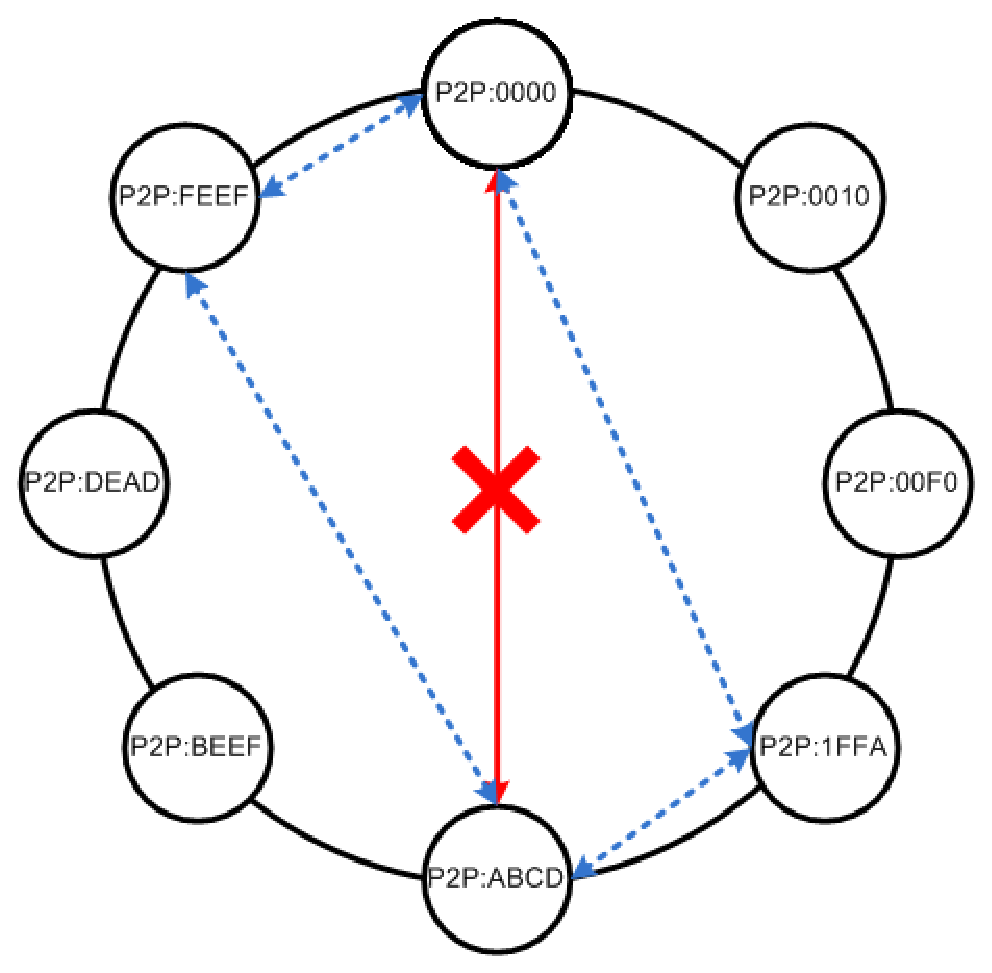
\epsfig{file=figs/relay.png.eps, width=3in}
\caption{Creating relays from across the node address space, when direct
connectivity is not possible.  Two members, 0000 and ABCD,  desire a direct
connection but are unable to directly connect, perhaps due to NATs or firewalls.
They exchange neighbor information through the overlay and connect to one of
each other's neighbors, creating overlap.  The overlap then becomes a a dedicated
relay path (represented by dashed lines), improving performance over relaying
across the entire overlay.}
\label{fig:relay}
\end{figure}

An additional feature added was the ability to exchange arbitrary information
along with the neighbor list.  So far we have implemented systems that pass
information about stability, via the age of a connection, and proximity, based
upon ping latency to neighbors.  Additionally, when overlap changes, we make
it optional to select to use only a subset of the overlap, thus only the
fastest or most stable overlap be used with many more in reserve.

To verify the usefulness of two-hop over overlay routing when direct connectivity
is not possible, we performed experiments and share the results in Section~\ref{relay_motivation}.
We also present some initial comparing our methods for selecting relays, age and latency,
in Section~\ref{relay_eval}.

\subsection{Bootstrapping Private Overlays}
In P2P systems, distributed security cannot provide the same level of security
as centralized or managed security.  Hopefully securing an overlay using
well-known security concepts such as PKI and SSL will encourage
wider adoption of P2P systems.  One problem with this approach though is that
users who want a private overlay may not have the resources, i.e. public
addresses, to host there own overlays.  To address this, we suggest
bootstrapping a private overlay from an existing public overlay.  The private
overlay will be completely encrypted and authenticated with only members of the
VPN allowed access.  This work is similar to previous in suggesting the use of
a public overlay to bootstrap application specific overlay has been discussed
in~\cite{one_ring}.

Members of the VPN are the only members of the overlay, providing a powerful
feature that the entire P2P overlay can be secured through groups.  This
prevents malicious users outside of the VPN from attacking it and more easily
enabled the removal of misbehaving peers, primarily rooted in the fact that
the use of a broadcast to signal a certificate revocation is now important to
the entire overlay.

The process for bootstrapping a private overlay follows.  Once the VPN software
begins, it starts by connecting with the public overlay.  It queries the public
overlay's DHT at the key ``private:groupname'', where groupname is the
GroupVPN's name.  The values stored at the key are the public overlay node IDs
of members actively in the private overlay.  The joining VPN software will
attempt to form private overlay leaf (bootstrap) connections with members of this
list over the public overlay.  During this process, both peers verify each
other's authenticity and form a secure connection.  This connection is then used
to bootstrap direct connections with members of the private overlay.  The reason
why the public overlay node IDs are stored at the public overlay's DHT key and
for using private overlay bootstrap connections over the public overlay is to
support NAT traversal.  This model allows reusing Brunets underlying NAT
traversal techniques to easily bootstrap private overlays.  As a member of a
private overlay, the VPN can somewhat more safely store information in the
private overlay's DHT, relegating the public overlay for private overlay
discovery.  Additionally, the public overlay could be used for relaying, when
direct connectivity is not possible, though this has not been looked into yet.

\section{Evaluation of VPN Models}
\label{evaluation}
For the purpose of quantitatively evaluation, we have added the features of
the proposed design parameters described in Section~\ref{p2pvpn} to IPOP
\cite{sc09} and Brunet~\cite{brunet}.  We present the advantage of using
relays over overlay routing when NAT traversal does not work.  Then we examine
the effects of using different relay selection mechanisms.  Afterwords, we
evaluate the system overheads of OpenVPN, Hamachi, and our P2P VPN to determine
the OS resource costs and the cost of each in a distributed environment.

\subsection{Motivation for Relays in the Overlay}
\label{relay_motivation}
The purpose of this experiment is to give weight to the argument that relays
are very useful for overlay networks that rely on low latency.  For this
experiment we applied the MIT King data set~\cite{king_data}, a data set
containing all-to-all latencies between 1,740 well-distributed Internet hosts.
We reviewed many different sizes of networks up to 1,740 nodes, evaluating each
network size 100 times.  Our experiments were executed in a simulator, where we
brought the system to steady state.  Once at steady state, we then calculate the average
all-to-all latency for all messages that would have taken two overlay hops
or more, the average of our low latency relay model, and the average of single
hop communication.  In the low latency relay model,
each destination node form a connection to the source nodes physically
closest peer as determined via latency (in a live system by application level
ping).  Then this pathway is used as a two-hop relay between source and node.
We only look at two overlay hops and more as a single hop would not necessarily
benefit from the work and would be the cause of a triangular inequality.

\begin{figure}[ht]
\centering
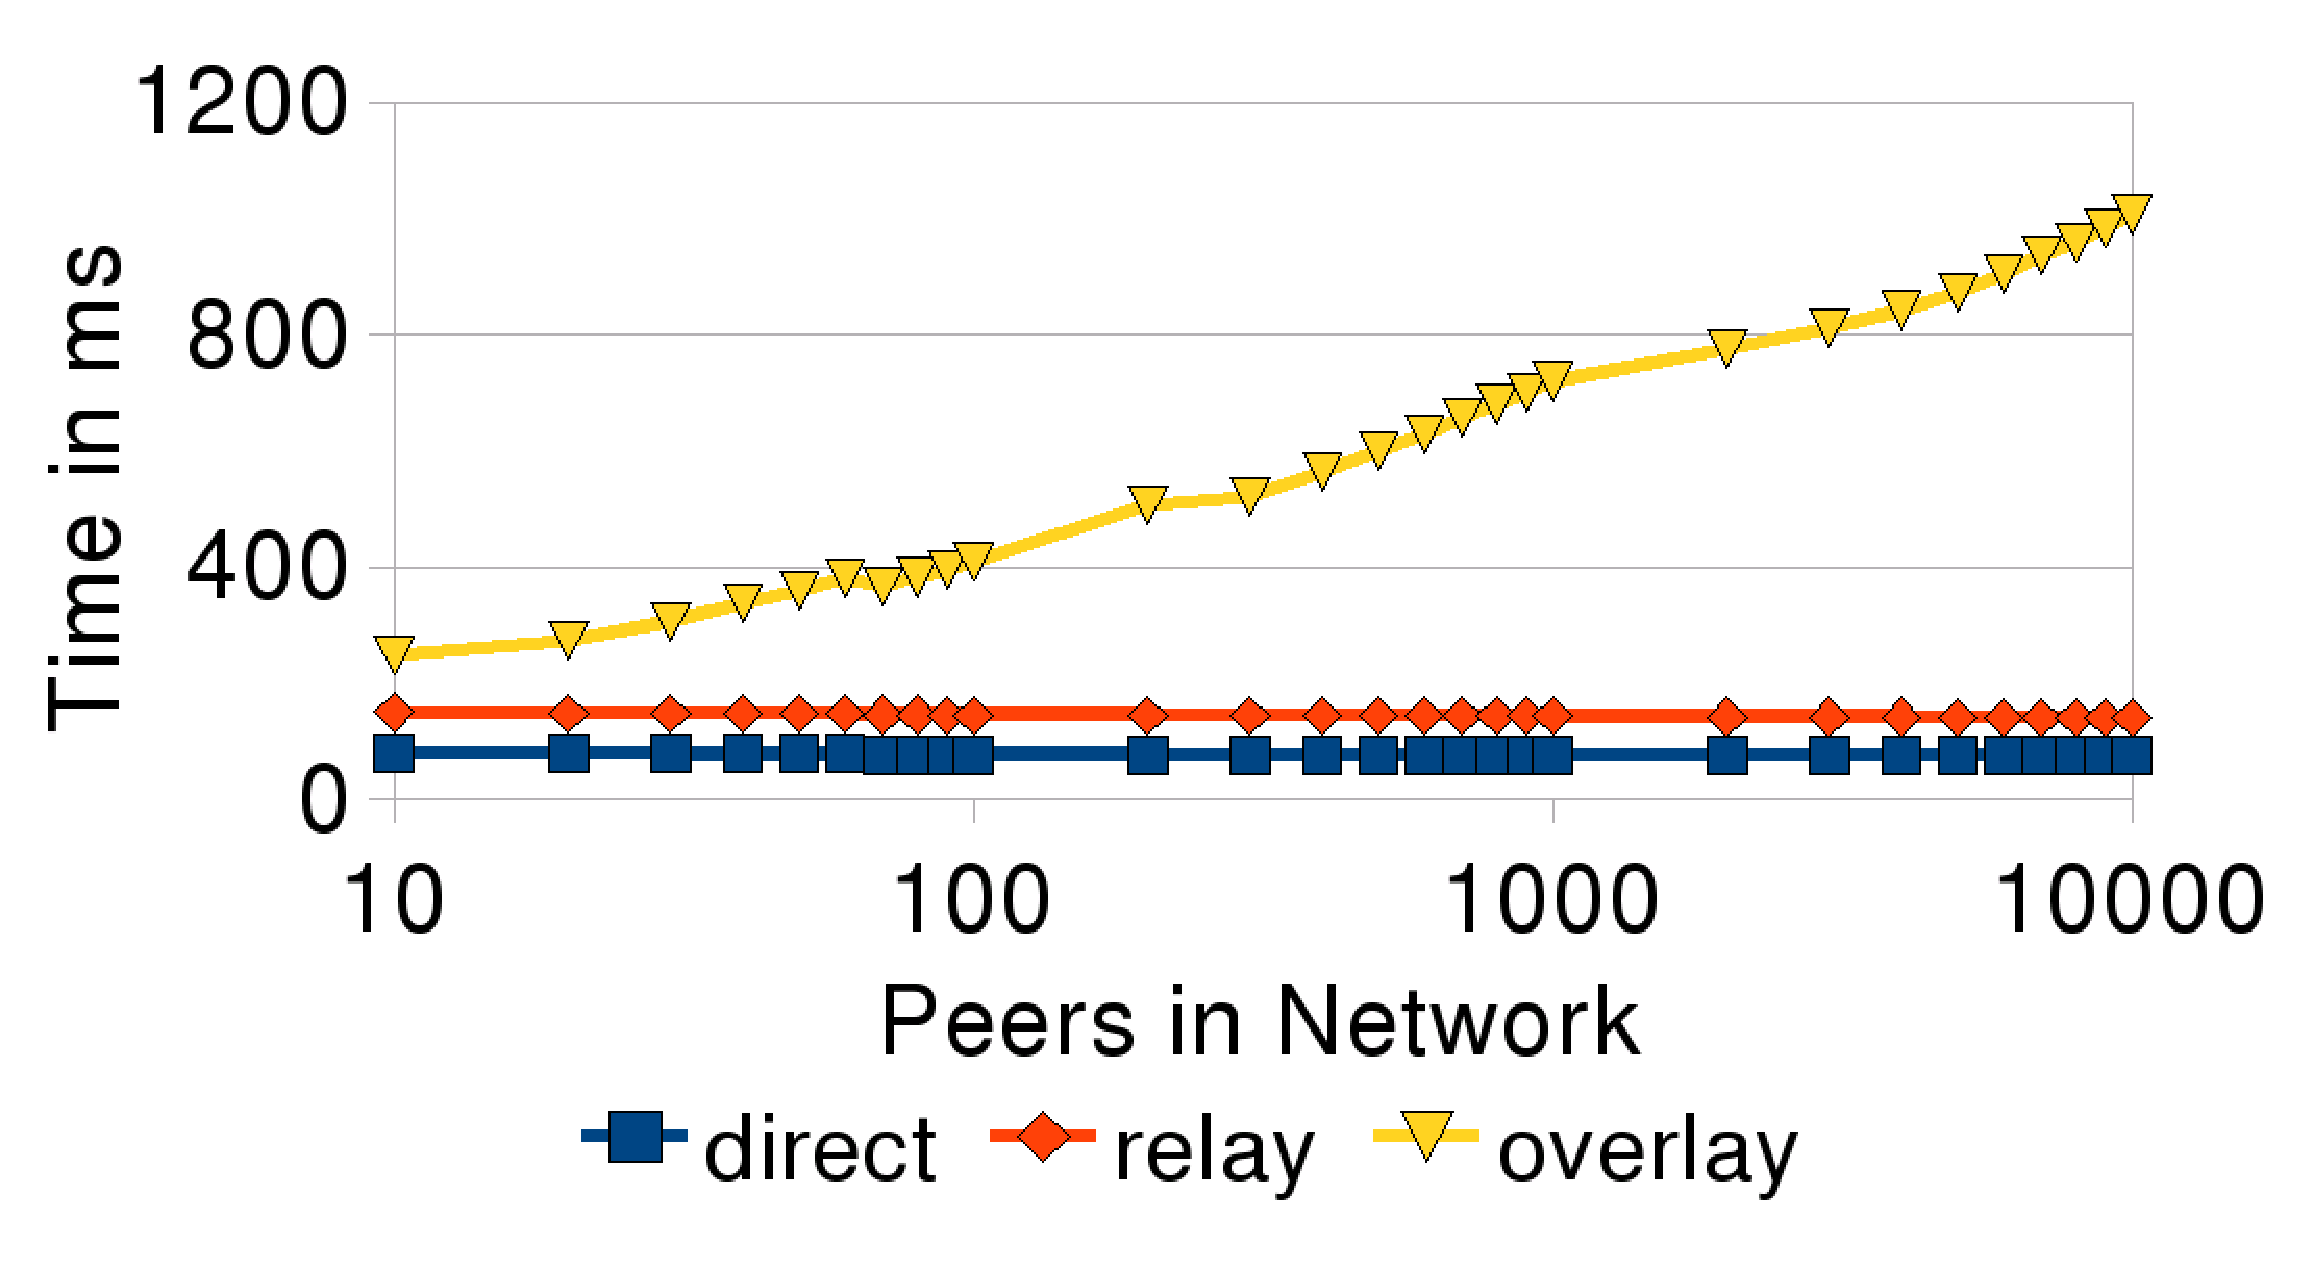
\epsfig{file=figs/relay_motivation.png.eps, width=3in}
\caption{A comparison of the average all-to-all overlay routing, two-hop relay, and
direct connection latency in a Structured P2P environment, Brunet, using the King
data set.}
\label{fig:simulated_relays}
\end{figure}

Our results are presented in Figure~\ref{fig:simulated_relays}.  We performed
the tests for varying network sizes.  We began our tests at 25, because network
sizes around 20 and under tend to be fully connected due to the connectivity
requirements of the system.  It is not until the network size expands past 100
and towards 200 nodes that two hop relays become significantly beneficial.  At
100 nodes, there is approximately an 54\% performance increase, whereas at
200 there is an 87\% increase and it appears to grow proportionately to the size
of the pool.  The key take away is that latency-bound applications
using a reasonably sized overlay would significantly benefit from
the use of two-hop relays.  Though as presented, it goes without saying that a two-hop
relay is not as fast as a direct connection.

\subsection{Comparing Relay Selection}
\label{relay_eval}
In this experiment, we evaluate time to establish a relays and measure bandwidth
and latency provided by the relays.  We perform the experiment on the Hamachi
relay selection as well as our two different models, latency and stability based.  The
setup for the experiment was two VPNs running on the same site but with
firewall, iptables, preventing direct communication.  We then start the VPN and
begin transmitting packets between the peers via Netperf~\cite{netperf}.  We time
how long it takes for a relay to form and then test for latency and bandwidth.
We repeated this test 100 times and present our results in Table~\ref{tab:relay_eval}.
To test latency, we used Netperf in TCP\_RR mode, where it performs a request-reply
between a client and a server.  Bandwidth is determined used Netperf in TCP\_STREAM
mode, which performs a bulk transfer between the client and server.

\begin{table}[ht]
\setlength{\itemsep}{0pt}
\setlength{\parskip}{0pt}
\centering
\begin{tabular}[c]{|m{2.2cm}||m{1.3cm}|m{1.3cm}|m{1.4cm}|} \hline
& Setup time (ms) & Latency (ms) & Bandwidth Mbit/s \\ \hline \hline
Hamachi & & & \\ \hline
Latency-aware & & & \\ \hline
Stability-aware & & & \\ \hline
\end{tabular}
\label{tab:relay_eval}
\caption{Results of the Relay evaluation comparing time to establish a relay,
bandwidth, and latency amongst Hamachi's relay service, a latency-focused relay
model, and an stability-focused relay model.}
\end{table}

The results look peculiar, but I can't figure out why.
\subsection{Comparing System Overheads}
In this experiment, we attempt to understand the bounds imposed by OpenVPN,
Hamachi, and IPOP.  We used Amazon EC2~\cite{ec2} to create various sized
networks ranging from 0 to 128 with additional client used as the control.
After boot, the each client places there IP address into a shared NFS direct,
once all client IP address are in the system, the bootstrap phase began.  In
the bootstrap phase, the control machine initiates communication with a
subset of clients in the VPN.  Once the system has warmed, we continue pinging
this subset every 15 seconds for the next 10 minutes.  We capture bytes
transmitted in to and out of the system as well as the memory size of the
VPN application at the end of each stage.  As we test the varying network
sizes, we begin by communicating with 0 peers and exponentially increase the
amount until the control is communicating with all members of the VPN.
For these evaluations, we purchased a Hamachi license, but due to very recent
changes in Hamachi, the Linux client will not support networks larger than 16.
Due to amount of data collected and space limitations, we only present Figures
for results that provide interesting data and summarize the rest in the text.

Memory followed, for the most part, an intuitive path, for each additional
connection there was more memory used.  The OpenVPN control client showed
negligible additional memory usage for additional nodes, though the server
showed a linear increment for each additional client in the system, around 1 MB
each, while activity had negligible effect on the results.  Hamachi had a
base line of a less than 1 MB and like OpenVPN, each additional client
in the system had a linear effect on memory, on the order of 4 KB, there was
no change based upon activity.  The effect of additional inactive nodes in
an IPOP network had negligible effect on memory, unlike Hamachi and OpenVPN.
The only time IPOP's memory consumption increased was during activity and it
scaled at a 200 KB per additional node.

\begin{figure}[ht]
\centering
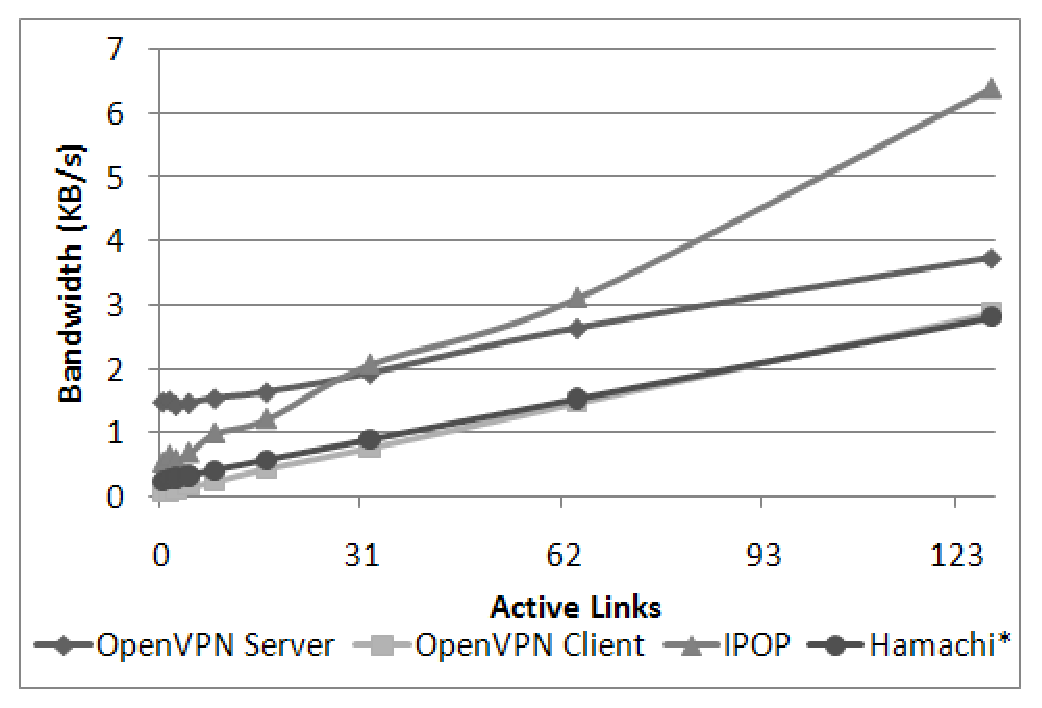
\epsfig{file=figs/bandwidth_128.png.eps, width=3in}
\caption{Comparison of bandwidth costs for member activity versus network size.
As stated in the text, Hamachi limits the system to network sizes of 16, so to
estimate the Hamachi bandwidth we used the following formula based upon a linear
regression model using our data sets: $.049 + .002 KB/s * N + .02 KB/s * A$,
.049 the bandwidth in a network size of 0, i.e., keep-alives with the central
server, N is the network size, and A is the active links.}
\label{fig:bandwidth_128}
\end{figure}

In Figures~\ref{fig:bandwidth_128}, we present our results for bandwidth for
client network sizes of 128.  Our evaluation scaled from having the control
communicate with 0 to 128 exponentially, though as mentioned already, Hamachi
only supports network sizes of 16, so we used a linear regression to extrapolate
the bandwidth results.  The results are somewhat predictable as Brunet, IPOP's
P2P infrastructure, primarily uses UDP connections and thus must maintain
application layer connections and actively ensures connections are open.
It is not obvious that Hamachi is doing the same, in fact, Hamachi's behavior
appears to be similar to that of OpenVPN.  OpenVPN does not need to maintain
bidirectional NAT mappings as the server is definitely on a public address,
thus a client does not need to be as proactive about ensuring the connection
is still alive as in IPOP and Hamachi.

The important take aways from this experiment are:  1) each additional member
in a VPN requires more memory, the structured P2P approach places this burden
only on the individual client and only when there is active communication,
2) maintaining NAT mappings along with negligible traffic (a ping every 15
seconds) requires very little bandwidth, and 3) all traffic routes through the
OpenVPN server and it pays a twice for each inter-client packet thus as
inter-client communication increases OpenVPN server's bandwidth will become a
bottleneck.

\section{Experiences}
\label{experiences}
Our work on the P2P VPN model presented in this paper is based on four
years of work spent developing, deploying, and maintaining VN software for
grid computing~\cite{wow,sc09,archer}.  In this section, we first present
our different deployments involving P2P VPN, then we present our experiences
in debugging a structured P2P system.

\subsection{Deployments}
Initially IPOP was designed to assist in self-configuring ad hoc grid deployments
using virtualization.  This can be seen in our project named ``Grid Appliance''
\cite{gridappliance}.  Over the year, the Grid Appliance has matured and so
has our usage of IPOP.  Currently, the Grid Appliance is used as the basis
for a free-to-join computer architecture consisting of over 400 compute resources
spanning 5 seed Universities with users across the United States and the World.
The Grid Appliances allows easy creation of ad hoc, distributed grids through
the use of the IPOP and the structured P2P DHT.  Experienced users can use the
system to create large grids in less than an hour with most of the time spent
waiting for virtual machines to boot.  Non-expert users can quickly access the
distributed grid in a matter of minutes by downloading a virtual machine
manager and the Grid Appliance.  The comment we receive most often in our
polls is ``I was surprised at how it just works.''

Motivation for a significant portion of our work lies in our desire to have non-Grid
Appliance connect to Grid Appliances resources in the same ``just works'' manner.
Thus bore our new incarnation of IPOP called GroupVPN, which now is the same
software stack that runs inside Grid Appliance but also allows services the Grid
Appliance to connect with external NFS and external grid resources.

Other work of ours' that relates to IPOP is the SocialVPN~\cite{cops08}.  The
SocialVPN places each client in their own private network, where they are only
addressable by their friends as defined by third party social network.
Unlike GroupVPN, this makes each user the master
of who does and does not have access to their resources.  Though this comes at
the cost of polling a central server, such as Facebook, to determine if a VPN
connection is legitimate, whereas the GroupVPN uses decentralized certificates
signed by a common CA.  SocialVPN does not lend itself well to environments
that require some form of central management such as a computing grid or a
small to medium businesses, for these purposes, we advocate GroupVPN.

\subsection{Discovering Faults}
In literature, the argument typically directed against structured P2P systems
is the ability to handle fault tolerance.  In this section, we share our
tactics for finding faults in a deployed overlay.

Our bootstrap system runs on Planet-Lab~\cite{planetlab}, placing it in that
harsh environment ensures that the system is reliability, stability, and
consistent.  Consistency compares peers knowledge of the pool and tests
each peer for congruence with both its first and second left and right neighbors.
We call this a crawl.  This information is stored in a database, which we can
later use to find nodes that have been inconsistent many consecutive times.
If a node is able to fix inconsistencies in future crawls, experience suggests
the inconsistency was probably due to churn in the system.  Otherwise, it will
probably still be in an inconsistent state and we are able to query the node
and other nodes nearby for additional state information.  At a minimum, this
would be help us determine if there exists a problem and potentially what state
is stale and causing the connectivity issue.  If this reveals little
information, we either retrieve a log or request it from the user who owns node,
the log typically provides some useful information.  Additionally, as with all
multithreaded applications, deadlocks happen, we found it useful to add
liveness states to threads to assist in finding deadlocks.

Other information, we watch, includes peer count, memory, and CPU usage.
Node count can be quite difficult to keep track of in Planet-Lab as machines at
a rate of 5 to 20 per day are restarted and our software is not automatically
restarted on these machines, thus the case to watch for is non-linear loss of
nodes.  Planet-Lab also places challenges on memory, as the systems can often be
I/O starved causing what appears to be memory leaks as Brunet's internal queue
can grow without bound.  In these cases, we have the node disconnect from the
overlay and sleep before returning.  The advantage of Planet-Lab as a test ground
is that it presents so many unique situations that can be very difficult to
reproduce in a lab controlled test system.  It is our belief
that any system that uses large scale Planet-Lab deployments as a testing ground
will be quite reliable.

We are still actively seeking better ways to verify the state of our system.
For example, the cost of doing a crawl can take $O(N \log(N))$ time,
since we have to communicate with every single node with an average routing
time of $O(\log(N))$.  For example, current research on Brunet has been focused
on providing a P2P MapReduce~\cite{mapreduce} framework, which can be used to
provide system wide searches and status checks in $O(\log(N))$ time.

\section{Related Works}
\label{related_work}
Our work is not the first to propose using a group like mechanism for regulating
member in a VPN, Hamachi presently offers the ability to create and join a
network from either a VPN client or through their website.  To create a group,
a user can either form a private invite only VPN or a password protected public VPN.
User's must exchange out of band both the password and the VPNs name and both
registered and unregistered users (guest) can join Hamachi VPNs.  Also, Hamachi
uses a key distribution center (KDC) as opposed to a PKI, thus it is quite
easy for Hamachi to do man-in-the-middle attacks.  Hamachi's server is not
redistributable and all user's must use LogMeIn's (Hamachi's owner) KDC and relays.
Our model ensures that each user is traceable and has to be authenticated by the
group administrator.  Groups entrance is further secured by giving each user a
unique key to retrieve signed certificates.  Most importantly our PKI is open
and redistributable, so user's can self-host, and our relays are built into the
VPN and require no management.

Our group system is not the first to provide an automatic PKI, previous work in
this field includes RobotCA~\cite{robotca}.  RobotCAs receive requests via e-mail,
they verify that the e-mail and the embedded PGP key match and sign the request.
RobotCAs are only as secure as the underlying e-mail infrastructure and provide
no guarantees about the person beyond their ownership of an e-mail address.  In
certain cases, this model could be used in our use cases, such as a SMB or handful
of universities that enforce all users to use university e-mails, then the RobotCA 
would only only sign e-mails, if they come from a specific domain.  Our experience
suggests that is not rare for an academic to use a non-university e-mail for
university purposes.  Another concern is that the RobotCA would require management
to limit allowed users to members of a class or an organization whose e-mail
addresses do not contain domain names.

VINI~\cite{vini}, an network infrastructure for evaluating new protocols and
services, uses OpenVPN along with Click~\cite{click} to provide access
from a VINI instance to outside hosts, as an ingress mechanism.  OpenVPN only
supports a single server and gateway per a client
and does support distributed load balancing.  VINI may benefit from using a
VPN that uses a full tunnel model similar to the our's as it lends itself
readily to interesting load balancing schemes.

\subsection{P2P VPN in Other Structured Overlays}
The purpose of this work is to develop a P2P VPN model that can easily be
applied to other structured P2P systems.  In this section, we focus on the
portability of our platform to other structured P2P systems, namely
Pastry and Chord by analyzing FreePastry and
NChord respectively.  FreePastry can easily reuse our C\# implemented
library through the use of IKVM.NET, which allows the porting of
Java code into the CLR.  NChord is a Chord implementation written in C\#.  In
Table~\ref{tab:structured_p2p_compare}, we compare the features of the structured
P2P systems as they apply to the use as a VPN.

\begin{table*}[!h!t]
\setlength{\itemsep}{0pt}
\setlength{\parskip}{0pt}
\centering
\begin{tabular}[c]{|m{2cm}||m{2.75cm}|m{2.8cm}|m{2.95cm}|m{1.65cm}|m{1.65cm}|} \hline
System & Overlay messaging & NAT Traversal & DHT & Secure PtP & Secure EtE\\ \hline
Brunet & Yes (AHSender) & UDP and overlay relaying & Yes with reliability & Yes & Yes \\ \hline
FreePastry & Yes (route) & Only with port-forwarding enabled  & Yes, PAST~\cite{past}, reliable & No & No \\ \hline
NChord & No, only look up & No & Simple, non-fault tolerant DHT & No & No \\ \hline
\end{tabular}
\caption{A comparison of structured P2P systems.  PtP stands for point-to-point
communication, such as communication between physical connections in a P2P
overlay.  EtE stands for end-to-end communication, such as messages routed
over the overlay between two peers.}
\label{tab:structured_p2p_compare}
\end{table*}

The bootstrapping of a connection in NChord, begins by finding the owner of the
DHT key containing the mapping of virtual IP address to node address
through ``find\_successor''.  After establishing a connection, the owner of the
key needs to be queried for the key's value, which would be the node ID of the
node owning the virtual IP.  After executing ``find\_successor'' and retrieving
the destination nodes, the owner of the virtual IPs, physical IP address, the VPN
can ``connect'' to the remote node using either a UDP or TCP socket.  Virtual IP
messages would then be sent and received through this ``connection''.  Unlike
other systems, NChord does not support sending messages through the overlay,
thus a separate ``connection'' for application purposes will need to be
created.

The steps involved in FreePastry begin by looking up the mapping of virtual
IP to node ID in PAST.  The result will be a node ID, which can be called
using ``route'' to send packets and ``deliver'' to handle incoming packets.
In fact, the model is very similar to Brunet.  Furthermore,  FreePastry has
knowledge of proximity in shortcuts, so it may be very easy to apply
high-performance autonomic relays to pastry.  FreePastry does not have
the ability to form shortcuts based upon demands, so if two peers were
actively communicating, they may always have to route traffic over the
overlay, which will probably be significantly slower than if they were
directly connected.  Though one could argue, that since FreePastry does
not support NAT traversal, all nodes will already be public and thus an
application, as in the NChord example, could form a direct connection bypassing
the overlay.

\section{Conclusions}
\label{conclusions}
This paper presents a novel VPN approach that has been designed from the ground up
to facilitate ease of use while maintaining a reasonable level of security.  At
the core of the VPN is a structured P2P system that provides decentralized
peer discovery, NAT traversal, relays, full tunnel gateways, and secure point-to-point
(PtP) and end-to-end (EtE) links.  The PtP and EtE links are secured via an group system
using a partially automated PKI with an intuitive web interface.  The web interface can
be hosted by the group themselves or they may use our public system~\cite{gridappliance}.

Through the use of the group interface, users can create their own VPNs with
private P2P pools while using public pools as a bootstrap.  Users are able to join
the system by downloading a stock VPN and loading it with their binary blob.  The
VPN will automatically connect to the appropriate web server and both parties will
verify each other's authenticity.  The user is then quickly connected to the VPN.
Administrators are able to police the system through the web interface and
offending users are eventually removed from the system through one of the following
mechanisms: CRL, DHT events, and broadcast messages.

The paper introduces many new interesting research problems: 1) distributed load 
balancing full tunnel gateways, 2) understanding the long term effects of different
automatic relay selection models, 3) understanding the benefits beyond security
of using a private overlay for a VPN.  We believe that this work provides both a
position and a model on how to design VPNs.

\bibliographystyle{abbrv}
%\small {
\bibliography{nsdi10}
\suppressfloats
%}

\end{document}
